\section{Numerical simulations}\label{Section5}

In this section, we will present several examples in which we solve our optimal control problem through the direct method and the non-linear constrained optimization tool \texttt{CasADi} \cite{Andersson2019}.
%
\subsection{Smooth approximation of piece-wise linear penalization}

With the final aim of using an optimization software to solve our optimal control problem, we will approximate our piece-wise linear penalization with the help of the Heaviside function $h:\mathbb{R} \rightarrow \mathbb{R}$ and its smooth approximation defined as follows: 
\begin{gather}
    h(x) = \begin{cases}
        1 & \text{ if } x \geq 0 \\
        0 & \text{ if } x < 0
    \end{cases}    
    \hspace{2em} 
    \begin{cases}
        h^\eta(x) = (1 + \tanh(\eta x))/2   \\
        \eta \rightarrow \infty
    \end{cases}
\end{gather}
Using $h$, we can define the (smooth) function $\Pi_{a,b}^\eta:\mathbb{R} \rightarrow \mathbb{R}$ as:
\begin{align*}
    \Pi_{[a,b]}^\eta(x) &= - 1 + h^\eta(x-a) + h^\eta(-x+b) 
    \\
    &= \frac{\tanh[\eta( x -a)] + \tanh[\eta (b-x)]}{2}.
\end{align*}
In this way, we can define the smooth version of \eqref{PLP}:
\begin{gather}
    \mathcal{L}^\eta(u) = \sum_{k = 1}^{N_u-1} \big[ (u_{k+1}+u_{k}) (u-u_k) + u_k^2 \big] \Pi^\eta_{[u_k,u_{k+1}]}(u)
\end{gather}
So that, when $\eta \rightarrow \infty$, then $\mathcal{L}^\eta \rightarrow \mathcal{L}$.

\subsection{Direct method  for  OCP-SHE}

To solve the optimal control problem (\ref{OCP2}), we use a direct method. 
%
If we consider a partition $\mathcal{P} = \{\tau_0,\tau_1,\dots,\tau_{T}\}$ of interval $[0,T]$ , we can represent a function $\{ u(\tau) \ | \ \tau \in [0,T]\}$ as a vector $\bm{u} \in \mathbb{R}^{T}$ where component $u_t = u(\tau_t)$. 
%
Then the optimal control problem (\ref{OCP1}) can be written as optimization problem with variable $\bm{u} \in \mathbb{R}^{T}$. This problem is a nonlinear programming, for this we use CasADi software to solve. 
%
Hence, given a partition of the interval $[0,\pi)$, we can formulate the problem \ref{OCP2} as the following one in discrete time
\newline

\begin{problem}[Numerical OCP]
Given two sets of odd numbers $\mathcal{E}_a$ and $\mathcal{E}_b$ with cardinalities $|\mathcal{E}_a| = N_a$ and $|\mathcal{E}_b| = N_b$ respectively, given the target vectors $\bm{a}_T  \in \mathbb{R}^{N_a}$, so that $\bm{x}_0 = [\bm{a}_T,\bm{b}_T]^T$ and $\bm{b}_T \in \mathbb{R}^{N_b}$ and a partition $\mathcal{P}_\tau = \{\tau_0,\tau_1,\dots,\tau_{T}\}$ of the interval $[0,\pi)$, we search a vector $\bm{u} \in \mathbb{R}^{T}$ that minimizes the following function:
\begin{gather}
        \min_{\bm{u} \in \mathbb{R}^{T} } 
        \Bigg[ 
        || \bm{x}^{T}||^2
        + \epsilon  \sum_{t=0}^{T-1} \mathcal{L}^\eta(u_{t}) \Delta\tau_t  \Bigg]  \\
        \notag \text{suject to: } \\
        \forall \tau \in \mathcal{P} \begin{cases}
            \bm{x}^{t+1} = \bm{x}^{t} - (2/\pi)\Delta \tau_t \bm{\mathcal{D}}(\tau_t)u_t \\
            \bm{x}^0 = \bm{x}_0
        \end{cases} 
\end{gather}
\end{problem}

\subsection{Resultados}

All our simulations have been performed with a laptop with $8Gb$ of RAM memory and the execution time for finding the solution given a target vector is os the order of $1s$. IN what follows, we will discuss all the numerical results we have obtained
\begin{enumerate}    
    \item \textbf{OCP with quarter-wave symmetry}: we will consider the problem with a set of odd numbers $\mathcal{E}_b = \{1,5\}$ and a discretization of $[0,\pi/2]$ with $T = 200$. We show the solutions for the target vectors $b_T^1 = \{(-0.4,-0.3,\dots,0.3,0.4)\}$ keeping $b_T^5=0$ for each case. We display the optimal trajectories we obtained in Figure \ref{ex01}, where we can see a continuity of the solutions with respect to the target vector.

    % \begin{figure}
    %     \centering
    %     \begin{subfigure}[b]{\textwidth}
    %         \centering
    %         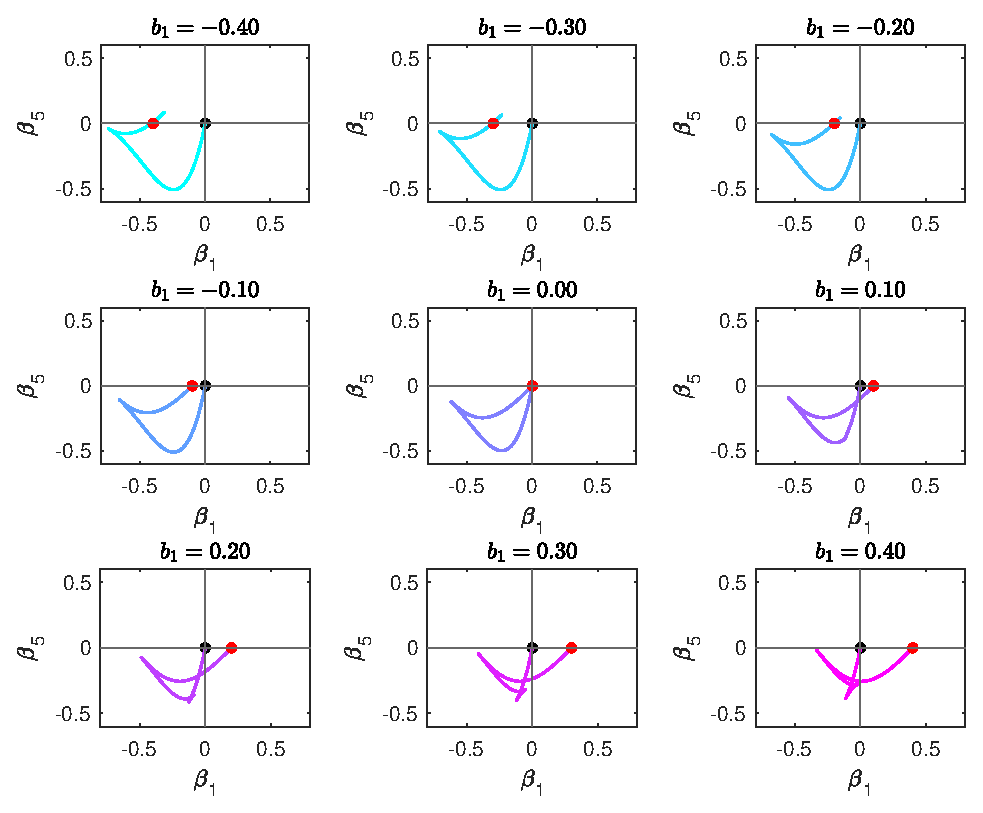
\includegraphics[width=0.6\textwidth]{img/ex01-con.eps}
    %         \caption{Dynamical System: el punto rojo hace referencia al punto final mientras que el punto negro hace referencia al punto inicial.}
    %     \end{subfigure} 
    %     \hfill \\
    %     \begin{subfigure}[b]{\textwidth}
    %         \centering
    %         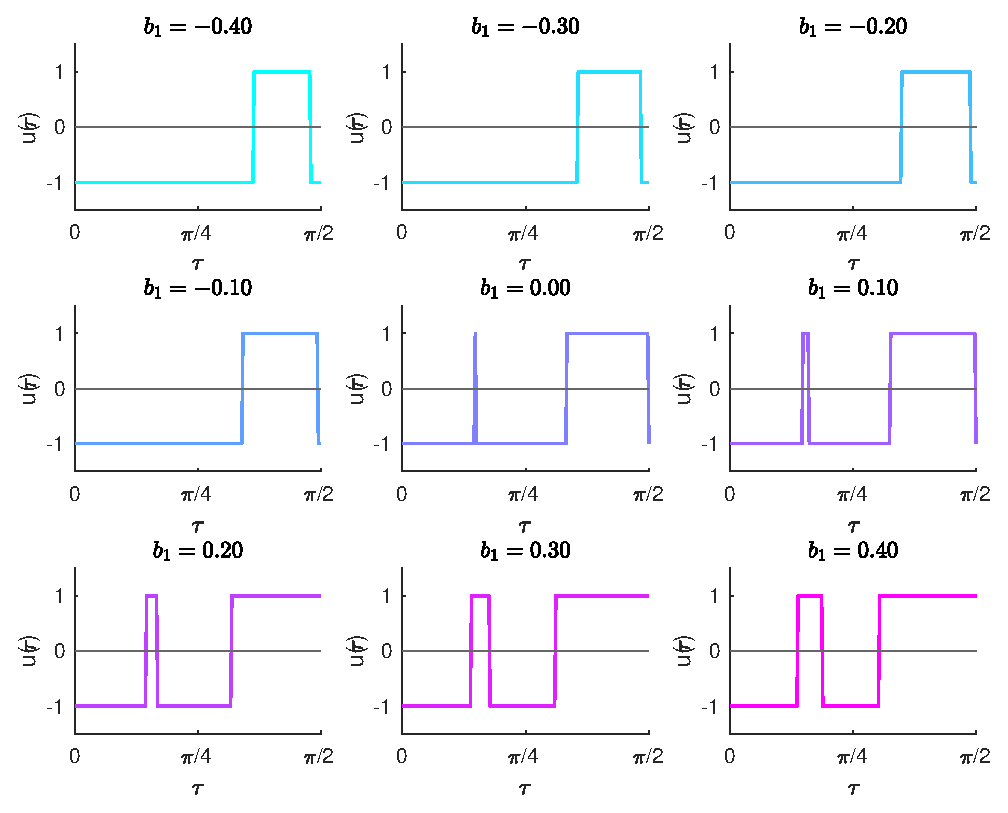
\includegraphics[width=0.6\textwidth]{img/ex01-dyn.eps} 
    %         \caption{Control}
    %     \end{subfigure}
    %     \caption{Mostramos las trayectorias óptimas y controles óptimos para distintos vectores objetivo.}
    %     \label{ex01}
    % \end{figure}


    \item \textbf{OCP with quarter-wave symmetry for an interval of $b_1$}: for this example we consider the following set of odd numbers: $\mathcal{E}_b = \{1,5,7,11,13\}$. 
    %
    Moreover, we consider the target vector $\bm{b}_T = [m_a,0,0,0,0]$, where $m_a \in [-1,1]$ is a parameter, with three penalization terms: $\mathcal{L}(u) = -f$, $\mathcal{L}(u) = +f$ and $\mathcal{L}(u) = -f^2$ obtained by direct method with uniform partition of interval $[0,\pi/2]$ with $T=400$ and penalization parameter $\epsilon = 10^{-5}$. 
    %
    For each one of the penalization terms we will employ, the distance between the Fourier coefficients is of the order $10^{-4}$. 
    %
    Nevertheless, when the penalization term is $\mathcal{L}(u)= -f^2$, the solution does not present continuity with respect to the target vector. 
    %
    On the other hand, it is important to mention that the solutions for the penalization terms $\mathcal{L}(u) = -f$ y $\mathcal{L}(u) = f$ are symmetric, so that inverting those solutions with respect to the origin and inverting their sign, it can be observed that they are the same.
     
    \item \textbf{SHE with three levels}: we can see that in the case in which the control $u(\tau)$ can only take values in $[0,1]$, we obtain signals which can take three levels in the interval $[0,2\pi]$ due to the quarter-wave symmetry. If we solve the optimal control problem this time with restrictions $\{0<u(\tau)<1\}$. We repeat the same procedure as before, thus obtaining solutions for the same penalization terms and obtaining Figure \ref{ex3LVL}. There we show the continuity of the solutions and that they are of the order $10^{-4}$.
    



    
      


    \item \textbf{Changes in the commutations number}: thanks to the optimal control formulation of SHE, we can vary the number of commutation angles. 
    %
    This is illustrated in the following example, where we considered the set of odd numbers $\mathcal{E}_b = \{1,3,9,13,17\}$. Moreover, we consider the target vector $\bm{b}_T = [m_a,0,0,0,0]$, where $m_a \in [0,1]$ is a parameter. 
    %
    In this problem, we used the penalization $\mathcal{L} = f$ with a penalization parameter $\epsilon=10^{-4}$.
    %
    We can see in Figure \ref{disco} that the optimal control problem is capable of moving among different solution sets.




    
    \item \textbf{OCP for SHE with half-wave symmetry}: we considered the optimal control problem in half-wave with $\mathcal{E}_a = \{1,3,5\}$ and  $\mathcal{E}_b = \{1,3,5,9\}$, where $\bm{a}_T = [m_a,0,0]$, $\bm{b}_T = [m_a,m_a,0,0]$ and $m_a \in [-0.6,0.6]$. We chose the penalization $L(u) = +f$



\end{enumerate}






